% !TeX root = ../skript.tex
% !TeX spellcheck = de_DE


\section{Lorenz-Modell}\label{lorenz-modell}
Die Gleichungen, welche das Lorenz-Modell beschreiben, enthalten viele physikalische Eigenschaften wie die Dichte, Geschwindigkeit und Temperatur der Atmosphäre. Lorenz wollte aus den bereits existierenden Gleichungen der Hydrodynamik ein Modell zur Wetterprognose erstellen. Basierend auf vorgehenden Arbeiten von Saltzman \cite{saltzman62} startete Lorenz mit den hyrodynamischen Gleichungen und verfolgte ein systematisches Näherungsvorgehen, womit er auf die folgenden drei Gleichungen stiess:

\begin{align}
\dot{x} &= \sigma(x - y)\\
\dot{y} &= x(\rho - z) - y\\
\dot{z} &= xy - \beta z
\end{align}

Die X-Achse entspricht dabei der hydrodynamischen, räumlichen Durchschnittsgeschwindigkeit, also die durchschnittliche Konvektionsgeschwindigkeit. Die Y-Achse repräsentiert die Temperatur und die Z-Achse der Temperaturgradient. Also wie schnell sich die Temperatur verändert. 

Wie aus den obigen Gleichungen ersichtlich ist, sind drei Parameter vorhanden. Alle sind immer positiv.

\subsubsection{1. Parameter: $\sigma$}
$\sigma$ entspricht der dimensionslosen Prandtl Zahl. Diese ist das Verhältnis von \textit{Viskosität} und der \textit{Wärmeleitfähigkeit}. Da beide Eigenschaften die Einheit $\frac{\text{m}^2}{\text{s}}$ haben, resultiert daraus eine dimensionslose Zahl.

\subsubsection{2. Parameter: $\rho$}
Dieser Parameter ist nach dem Physiker Baron Rayleigh benannt worden und heisst Rayleigh Zahl. Es entspricht dem Verhältnis von \textit{Wärmeausdehnung} und der \textit{Viskosität}.

\subsubsection{3. Parameter: $\beta$}
Das $ \beta $ entspricht der \textit{Wärmeausdehnung}. Dabei handelt es sich um die Veränderung der geometrischen Abmessungen (Länge, Flächeninhalt und Volumen) eines Körpers, die sich mit erhöhter Temperatur vergrössern.

\begin{figure}
	\centering
	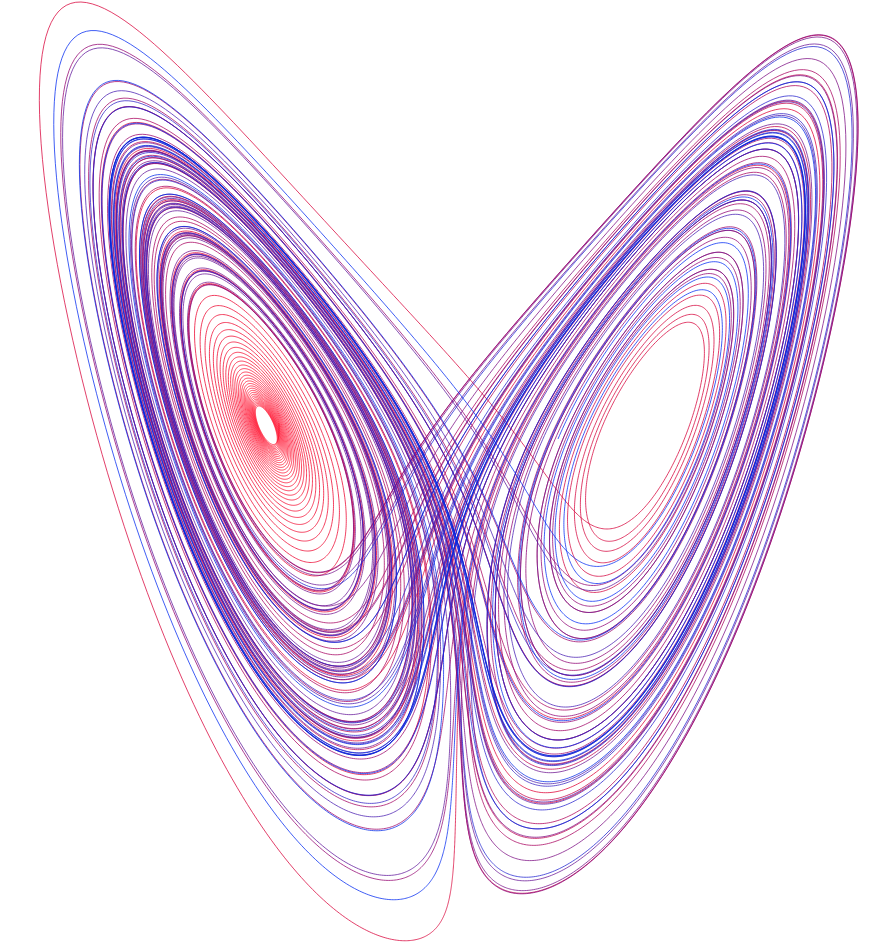
\includegraphics[width=0.3\linewidth]{lorenz/assets/lorenz-modell/lorenz-modell}
	\caption{Bahn des Lorenz-Modell mit $\rho = 28$, $\sigma = 10$ und $\beta = \frac{8}{3}$}
	\label{fig:lorenz-modell}
\end{figure}


\subsection{Numerische Lösungen}
Es gibt für das Lösen von Differentialgleichungen zwei Ansätze. Zum einen der analytische Ansatz, der eine allgmeingültige Lösung sucht. Es handelt sich bei den drei Lorenz-Gleichungen um nicht-lineare Differentialgleichungen, welche analytisch nicht lösbar sind. Aus diesem Grund fällt dieser Lösungsweg weg. 

Der zweite Ansatz ist, eine \textit{Diskretisierung} vorzunehmen und den Computer für jeden definierten Zeitpunkt die Resultate der Gleichungen \textit{numerisch} ausrechnen zu lassen. Dies ist auch der in dieser Arbeit gewählte Weg, der im Folgenden bis zur tatsächlichen Visualisierung genauer beschrieben wird.

\subsubsection{Euler-Verfahren}

Wir wählten für die Diskretisierung das \textit{Euler-Verfahren} zur Annäherung der Werte des Lorenz-Modells. Das resultierende Gleichungssystem besteht aus einfachen Arithmetik-Operationen und ist für einen Computer einfach berechenbar. Dies erlaubt auch \textit{Smartphones} die Visualisierung effizient zu berechnen und flüssig anzuzeigen.

Das Euler-Verfahren ist ein Algorithmus der Familie der Einschritt-Verfahren. Diese Verfahren rechnen schrittweise die Werte von einem Startwert aus. Sie können dies in einer $ O(N) $ Schleife bei welcher die Lösung des vorherigen Durchgangs als neuer Startwert verwendet wird. 

Differentialgleichungen beschreiben die Steigung relativ zu bekannter Lösung. Sie sagen nichts über die X-Achsen-Verschiebung der Werte aus. Aus diesem Grund kennt man die absolute Position dieser Werte nicht und kann auch keine andere Positionen daraus ausrechnen. Der vorhergehend vorgestellte Algorithmus kann lediglich die anderen Werte ausrechnen wenn dieser Startwert im vorhinein bekannt ist. Dieses Hindernis wird das \textit{Anfangswert-Problem} genannt.

Auch das besprochene Verfahren kann das Anfangswert-Problem nicht lösen, sondern nur schrittweise vom Anfangswert die anderen Punkte ausrechnen. Wir haben diese Problematik im Rahmen dieses Berichtes nicht lösen können und stattdessen den Anfangswert $ P(0.1, 0.1, 0.1) $ angenommen. Dieser Anfangswert war konstant und fester Teil des Algorithmus, den wir modeliert haben.

Wir versuchten zuerst den Anfangswert $ P(0, 0, 0) $ zu nehmen. In den anschliessenden Untersuchungen des Algorithmus stellte sich heraus, dass dieser Anfangswert zugleich eine Lösung des Lorenz-Systems ist. Aus diesem Grund hat sich das Model auf den Ursprung stabilisiert. Unsere Lösung war es den Anfangswert auf $ P(0.1, 0.1, 0.1) $ zu verschieben, der diese Eigenschaft nicht besitzt.

Als Basis für das Euler-Verfahren verwenden wir den Differenzenquotient $ \frac{dx}{dt} \approx \frac{x_{n + 1} - x_n}{\Delta t} $ \cite{euler1768}.  Weil wir den nächsten Punkt im 3D-Raum ausrechnen möchten, formen wir die Gleichung zu $ x_{n + 1} $  um und rechnen sie für alle Achsen getrennt aus.

\begin{align}
    x_{n + 1} &= x_n + \frac{dx}{dt} \cdot \Delta t\\
    y_{n + 1} &= y_n + \frac{dy}{dt} \cdot \Delta t\\
    z_{n + 1} &= z_n + \frac{dz}{dt} \cdot \Delta t
\end{align}

% TODO Neuschreiben, detailhafter
Für die Ableitungen können wir nun die Gleichungen des Lorenz-Modells einsetzen. Die Variablen $ x, y, z $ haben wir ausserdem zu Iterationsvariablen 
\begin{align}
    x_{n + 1} &= x_n + \sigma(x_n - y_n) \cdot \Delta t\\
    y_{n + 1} &= y_n + x_n(\rho - z_n) - y_n \cdot \Delta t\\
    z_{n + 1} &= z_n + (x_n \cdot y_n - \beta \cdot z_n) \cdot \Delta t
\end{align}

Dieses System entspricht dem Code der Visualisierung weiter unten. Im Differentialterm wurde die Differentialgleichung des Lorenz-Modells eingesetzt.
